\chapter{Introduction}
\section{What is Machine Learning}
Machine learning is a subfield of computer science that is concerned with building algorithms which to be useful, rely on a collection of examples of some phenomenon.
\begin{itemize}
	\item The examples come from nature, handcrafted by humans or generated by another algorithms.
\end{itemize}
Machine learning can also be defined as the process of solving a practical problem by
\begin{enumerate}
	\item gathering a dataset
	\item algorithmically building a statistical model based on the dataset.
\end{enumerate}
The statistical model is assumed to be used somehow to solve the practical problem.
\section{Types of Learninig}
Learning can be \textbf{supervised}, \textbf{semi-supervised}, \textbf{unsupervised} and \textbf{reinforcement}.
\subsection{Supervised Learning}
In \textbf{supervised learning}, the \textbf{dataset} is the collection of \textbf{labeled examples} $\left\{\left(\mathbf{x}_i, y_i\right)\right\}_{i=1}^N$.
\begin{itemize}
	\item Each element $\mathbf{x}_i$ among $N$ is called a \textbf{feature vector}. A feature vector is a vector in which each dimension $j=1,...,D$ contains a value that describes the example somehow. That value is called a \textbf{feature} and is denoted as \(x^{(j)}\).
	\item The \textbf{label} \(y_i\) can be either an element belonging to a finite set of \textbf{classes} ${1,2,...,C}$, or a real number, or a more complex structure, like a vector, a matrix, a tree or a graph. Unless otherwise stated, $y_i$ is either one of a finite set of classes or a real number.
\end{itemize}
The goal of a \textbf{supervised learning algorithm} is to use the dataset to produce a \textbf{model} that takes a feature vector $\mathbf{x}$ as input and outputs information that allows deducing the label for this feature vector.

\subsection{Unsupervised Learning}
In \textbf{unsupervised learning}, the dataset is a collection of \textbf{unlabeled examples} $\left\{\mathbf{x}_i\right\}_{i=1}^N$. The goal of an \textbf{unsupervised learning algorithm} is to create a model that takes a feature vector $\mathbf{x}$ as input and either transforms it into another vector or into a value that can be used to solve a practical problem. For example,
\begin{itemize}
	\item in \textbf{clustering}, the model returns the id of the cluster for each feature vector in the dataset.
	\item in \textbf{dimensionality reduction}, the output of the model is a feature vector that has fewer features than the input $\mathbf{x}$;
	\item in \textbf{outlier detection}, the output is a real number that indicates how $\mathbf{x}$ is different from a ``typical" example in the dataset.
\end{itemize}
\subsection{Semi-Supervised Learning}
In \textbf{semi-supervised learning}, the dataset contains both labeled and unlabeled examples.
\begin{itemize}
	\item Usually the quantity of unlabeled examples is much higher than the number of labeled examples.
\end{itemize}
The goal of \textbf{semi-supervised learning algorithm} is the same as the goal of the supervised learning algorithm.
\begin{itemize}
	\item The hope here is that using many unlabeled examples can help the learning algorithm to find a better model.
\end{itemize}
How does the learning benefit from adding more unlabeled examples?
\begin{itemize}
	\item By adding unlabeled examples, you add more information about your problem:\textit{ a larger sample reflects better the probability distribution the data we labeled came from}.
\end{itemize}

\subsection{Reinforcement Learning}
\textbf{Reinforcement learning} is a subfield of machine learning where the machine ``lives" in an environment and is capable of perceiving the \textit{state} of that environment as vector of features.
\begin{itemize}
	\item The machine can execute \textit{actions} in every state. Different actions bring different \textit{rewards} and could also move the machine to another state of the environment.
\end{itemize}
The goal of a reinforcement learning algorithm is to learn a \textit{policy}. A policy is a function (similar to the model in supervised learning) that takes the feature vector of a state as input and outputs an optimal action to execute in that state. The action is optimal if it maximizes the \textit{expected average reward}.

\section{How Supervised Learning Works}
Supervised learning is the type of machine learning most frequently used in practice. The supervised learning process starts with gathering the data. The data for supervised learning is a collection of pairs (input,output).
\begin{itemize}
	\item Inputs could be anything, for example, email messages, pictures, or sensor measurements.
	\item Outputs are usually real numbers, or labels (e.g. ``spam", ``not\_spam", etc). In some cases, outputs are vectors (e.g., four coordinates of the rectangle around a person on the picture), sequences (e.g. [``adjective", ``adjective", ``noun"] for the input ``big beautiful car") or have some other structure.
\end{itemize}
You want to solve spam detection using supervised learning. First, you gather the data of 10,000 email messages and you have your label ``spam" or ``not\_spam" for each message. With the data at hand, you have to represent each message using a feature vector.

A common approach it to use \textbf{bag of words}, is to take a dictionary of English words (e.g. 20,000 alphabetically sorted words) and stipulate that in our feature vector:
\begin{itemize}
	\item the first feature is equal to 1 if the email message contains the word ``a"; other wise, this feature is 0;
	\item the second feature is equal to 1 if the email message contains the word ``aaron"; otherwise, this feature equals 0;
	\item ...
	\item the feature at position 20,000 is equal to 1 if the email message contains the word ``zulu"; otherwise, this feature is equal to 0.
\end{itemize}
You repeat the above procedure for every email message in our collection, which gives us 10,000 feature vectors (each vector having the dimensionality of 20,000) and a label (``spam"/``not\_spam").

We successfully converted input data into machine-readable type, but the output labels are still in the form of human-readable text. Some learning algorithms require transforming labels into numbers. For demonstration purpose, we will use a supervised learning algorithm called \textbf{Support Vector Machine} (SVM). This algorithm requires the positive label (in our case it's ``spam") has the numeric value of +1 (one), and the negative label (``not\_spam") has the value of -1 (minus one).

You now have a \textbf{dataset} and a \textbf{learning algorithm}, you will need to apply the learning algorithm to the dataset to get the \textbf{model}.

SVM sees every feature vector as a point in a high-dimensional space (in our case, space is 20,000-dimensional). The algorithm puts all feature vectors on an imaginary 20,000-dimensional plot and draws an imaginary 19,999-dimensional line (a \textit{hyperplane}) that separates examples with positive labels from examples with negative labels. In machine learning, the boundary separating the examples of different classes is called the \textbf{decision boundary}.

Hyperplane is denoted by two \textbf{parameters}

\[ \mathbf{w} \mathbf{x}-b=0 \text {, } \]
\begin{itemize}
	\item a real-valued vector $\mathbf{w}$ of the same dimensionality as our input vector $\mathbf{x}$, and a real number $b$
	\item $\mathbf{w} \mathbf{x}= w^{(1)} x^{(1)}+w^{(2)} x^{(2)}+\ldots+w^{(D)} x^{(D)}$, and $D$ is the number of dimensions of the feature vector $\mathbf{x}$.
\end{itemize}
The predicted label for some input feature vector $\mathbf{x}$ is given like this:

$$
	y=\operatorname{sign}(\mathbf{w} \mathbf{x}-b),
$$

where \verb*|sign| is a mathematical operator that takes any value as input and returns $+1$ if the input is a positive number or $-1$ if the input is a negative number.

The goal of the learning algorithm, SVM in this case, is to leverage the dataset and find the optimal values \(\mathbf{w}^{*}\) and $b^{*}$ for parameters $\mathbf{w}$ and $b$. Once the learning algorithm identifies these optimal values, the \textbf{model} $f(\mathbf{x})$ is then defined as:

\begin{equation*}
	f(\mathbf{x})=\operatorname{sign}\left(\mathbf{w}^* \mathbf{x}-b^*\right)
\end{equation*}


How do we find these optima values? It turns out it is an optimization problem. Machines are good at optimizing functions \underline{under constraints}.

$$
	\begin{array}{ll}
		\mathbf{w} \mathbf{x}_{i}-b \geq+1 & \text { if } y_{i}=+1 \\
		\mathbf{w} \mathbf{x}_{i}-b \leq-1 & \text { if } y_{i}=-1
	\end{array}
$$

It will also be ideal if the hyperplane separates positive examples from negative ones with the largest \textbf{margin}. The margin is the distance between the closestt examples of two classes, as defined by the decision boundary. A large margin contributes to a better \textbf{generalization}, that is how well the model will classify new examples in the future.

\begin{figure}[H]
	\centering
	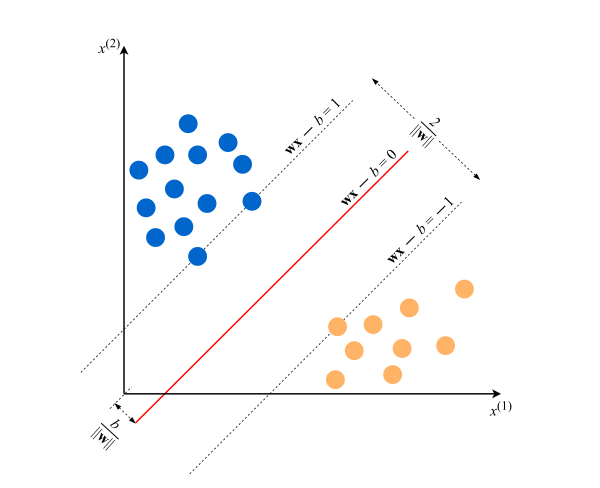
\includegraphics[width=0.7\linewidth]{imgs/introduction/intro_1}
	\caption{An example of an SVM model for two-dimensional feature vectors.}
	\label{fig:intro1}
\end{figure}

Let's do some quick refreshment
\vspace*{1em}
\begin{tcolorbox}[enhanced jigsaw, breakable, pad at break*=1mm, colback=gray!20!white, colframe=black!85!black, title=\textbf{Distance Formulas in Euclidean Space}]
	\textbf{Distance Between Two Points} \\
	In two-dimensional space, for points \( P_1(x_1, y_1) \) and \( P_2(x_2, y_2) \), the distance is calculated as:
	\[ d = \sqrt{(x_2 - x_1)^2 + (y_2 - y_1)^2} \]

	\textbf{Distance From a Point to a Line} \\
	In two-dimensional space, for a line defined by \( ax + by + c = 0 \) and a point \( P(x_0, y_0) \), the distance is:
	\[ d = \frac{|ax_0 + by_0 + c|}{\sqrt{a^2 + b^2}} \]

	\textbf{Distance Between Two Parallel Lines} \\
	For two parallel lines with equations \( ax + by + c_1 = 0 \) and \( ax + by + c_2 = 0 \), the distance is:
	\[ D = \frac{|c_2 - c_1|}{\sqrt{a^2 + b^2}} \]
\end{tcolorbox}
\vspace*{1em}
So, the optimization problem that we want the machine to solve looks like this:

\textit{\textbf{Minimize} $\|\mathbf{w}\|$ subject to $y_{i}\left(\mathbf{w} \mathbf{x}_{i}-b\right) \geq 1$ for $i=1, \ldots, N$. The expression $y_{i}\left(\mathbf{w} \mathbf{x}_{i}-b\right) \geq 1$ is just a compact way to write the above two constraints.}

More on SVMs later. This simple example should give you an idea how supervised learning works.

\section{Why the Model Works on New Data}

Let's refer to Figure \ref{fig:intro1}. If two classes are separable from one another by a decision boundary, then, obviously, examples that belong to each class are located in two different subspaces which the decision boundary creates.

If the examples used for training were selected randomly, independently of one another, and following the same procedure, then statistically, it is \textit{more likely} that the new negative example will be located on the plot somewhere not too far from other negative examples.  The idea goes with the positive examples as well.

